\documentclass[discrete.tex]{subfiles}

\begin{document}
  \section{Обходы графа в ширину и глубину. Топологическая сортировка}

  \begin{Alg}[обход в ширину]
    \[M = M_0 \cap M_1 \cap M_2\]
    $x_0$ - корень обхода (начальная вершина)\\
    $M_0$ - пройденные вершины\\
    $M_1$ - рассматриваемые\\
    $M_2$ - ещё не пройденные \\ \ \\
    Начальное состояние:
    \[M_0 = \varnothing\q M_1 = \{x_0\}\q M_2 = M \setminus M_1\]
    \[while\q (M_1 <> \varnothing)\]
    \begin{enumerate}
      \item Рассмотрим $x \in M_1$
      \item $\forall u \in N_x$ (дуги, инцедентные с x):
      \[\text{Рассмотрим }\End(u):\]
      \begin{enumerate}
        \item если $\End u \in M_0$: ничего не делаем
        \item если $\End u \in M_1$: ничего не делаем
        \item если $\End u \in M_2 \Ra \End u \ra M_1$
        и удаляем вершину из $M_2$
      \end{enumerate}
      \item $x \ra M_0$
    \end{enumerate}
  \end{Alg}

  \begin{example} \
    \begin{figure}[H]
            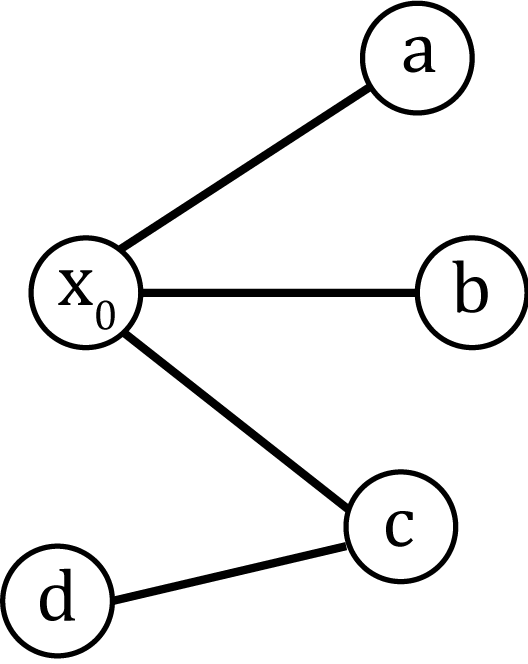
\includegraphics[width=3cm]{pics/38_1}
            \centering
    \end{figure}
    \begin{enumerate}
      \item $M_0 = \varnothing,\q M_1 = \{x_0\},\q M_2 = \{a,b,c,d\}$\\
      Рассмотрим $x_0$:
      \[U: a,b,c \ra M_1\]
      \[\q x_0 \ra M_0\]
      \item $M_0 = \{x_0\},\q M_1 = \{a,b,c\},\q M_2 = \{d\}$\\
      Рассмотрим a:
      \[u: x_0 \in M_0;\q a \ra M_0\]
      \item $M_0=\{x_0,a\},\q M_1 = \{b,c\},\q M_2=\{d\}$\\
      Рассмотрим b:
      \[u: x_0 \in M_0;\q b \ra M_0\]
      \item $M_0=\{x_0,a,b\},\q M_1 = \{c\},\q M_2 = \{d\}$\\
      Рассмотрим c:
      \[u: x_0 \in M_0\]
      \[d \in M_0 \Ra d \ra M_1\]
      \[c \ra M_0\]
      \item $M_0=\{x_0,a,b,c\},\q M_1 = \{d\},\q M_2 = \varnothing$\\
      Рассмотрим d:
      \[u: x_0 \in M_0,\q c \in M_0\]
      \[d \ra M_0\]
      \[\Ra M_0=\{x_0,a,b,c,d\}\]
      - перечисляем вергины от $x_0$ в порядке возрастания длин путей (числа ребер в пути)
    \end{enumerate}
  \end{example}

  \begin{alg}[алгоритм в глубину]
    $x_0$ - корень
    \[R(x_0,x_1,...,x_k) \text{ - радиус, нач. сост: }R(x_0)\]
    \begin{enumerate}
      \item Рассмотрим $u \in N_{x_k}$\\
      Если $\e$ неотмеченная $\us{\neq R(...)}{u}$, то
      \[\Ra R(x_0,...,x_k,\End(u))\]
      Если $\not \e$ неотмеченных $\Ra$ удаляем вершину $x_k$ и все инцидентные ей вершины
    \end{enumerate}
  \end{alg}

  \begin{example} \
    \begin{figure}[H]
            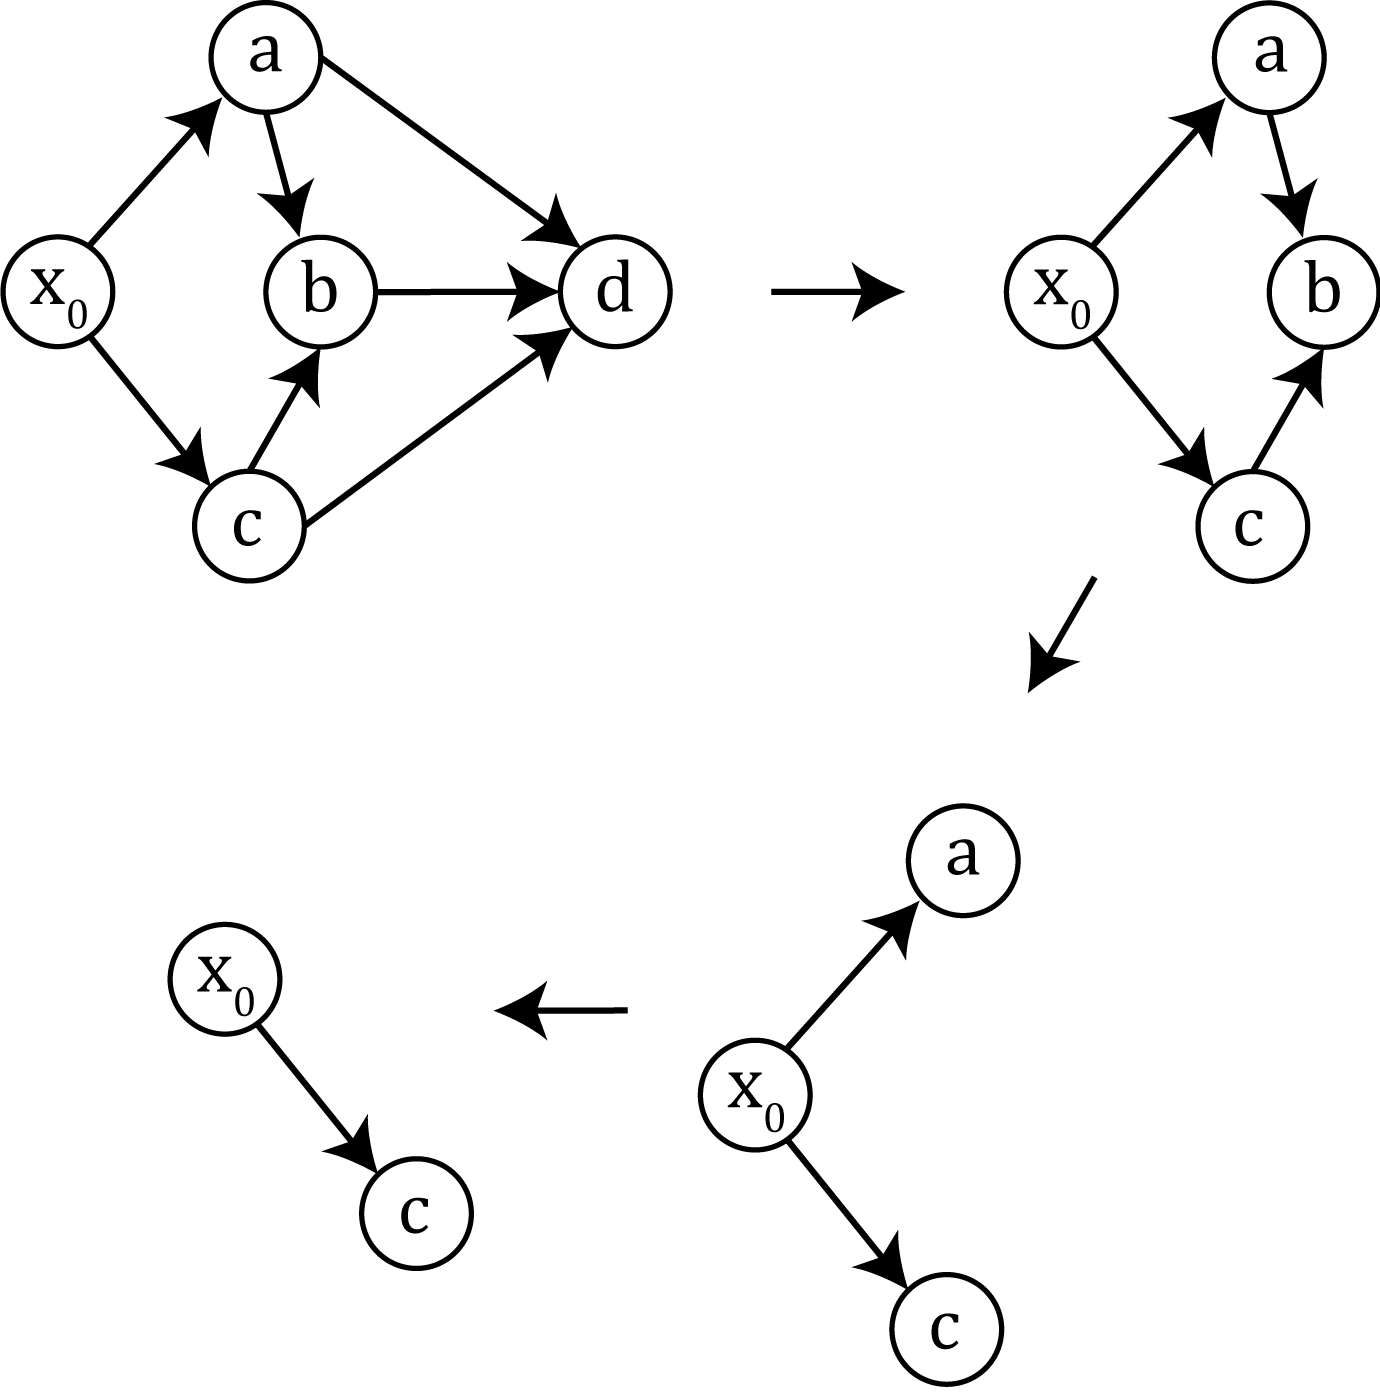
\includegraphics[width=5cm]{pics/38_2}
            \centering
    \end{figure}
    \[R(x_0)\]
    \[R(x_0,a)\]
    \[R(x_0, a, d) \text{: удаляем $d$ и $(b,d)$, $(a,d)$, $(c,d)$} \Ra R(x_0,a)\]
    \[R(x_0, a, d) \text{: удаляем $b$ и $(a,b)$, $(x_0,b)$, $(c,b)$} \Ra R(x_0,a)\]
    \[R(x_0,a) \text{: удаляем $a$ и $(x_0,a)$} \Ra R(x_0)\]
    \[R(x_0,c) \text{: удаляем $c$ и $(x_0,c)$}\]
    \[\Ra R(x_0) \text{: удаляем $x_0$}\Ra R(\varnothing)\]
  \end{example}

  \begin{alg}[топологическая сортировка]
    Применяется лишь к ориентированным графам без контуров
    \[N_i^+ \text{ - мн-во дуг, входящих в i}\]
    \[N_i^+ \text{ - мн-во дуг, выход из i}\]
    Рассмотрим вершину, которая $N_i^+ = \varnothing$\\
    Удаляем её $(\ra M_0)$ и удаляем все её $N_i^-$
  \end{alg}

  \begin{example}
    \begin{figure}[H]
            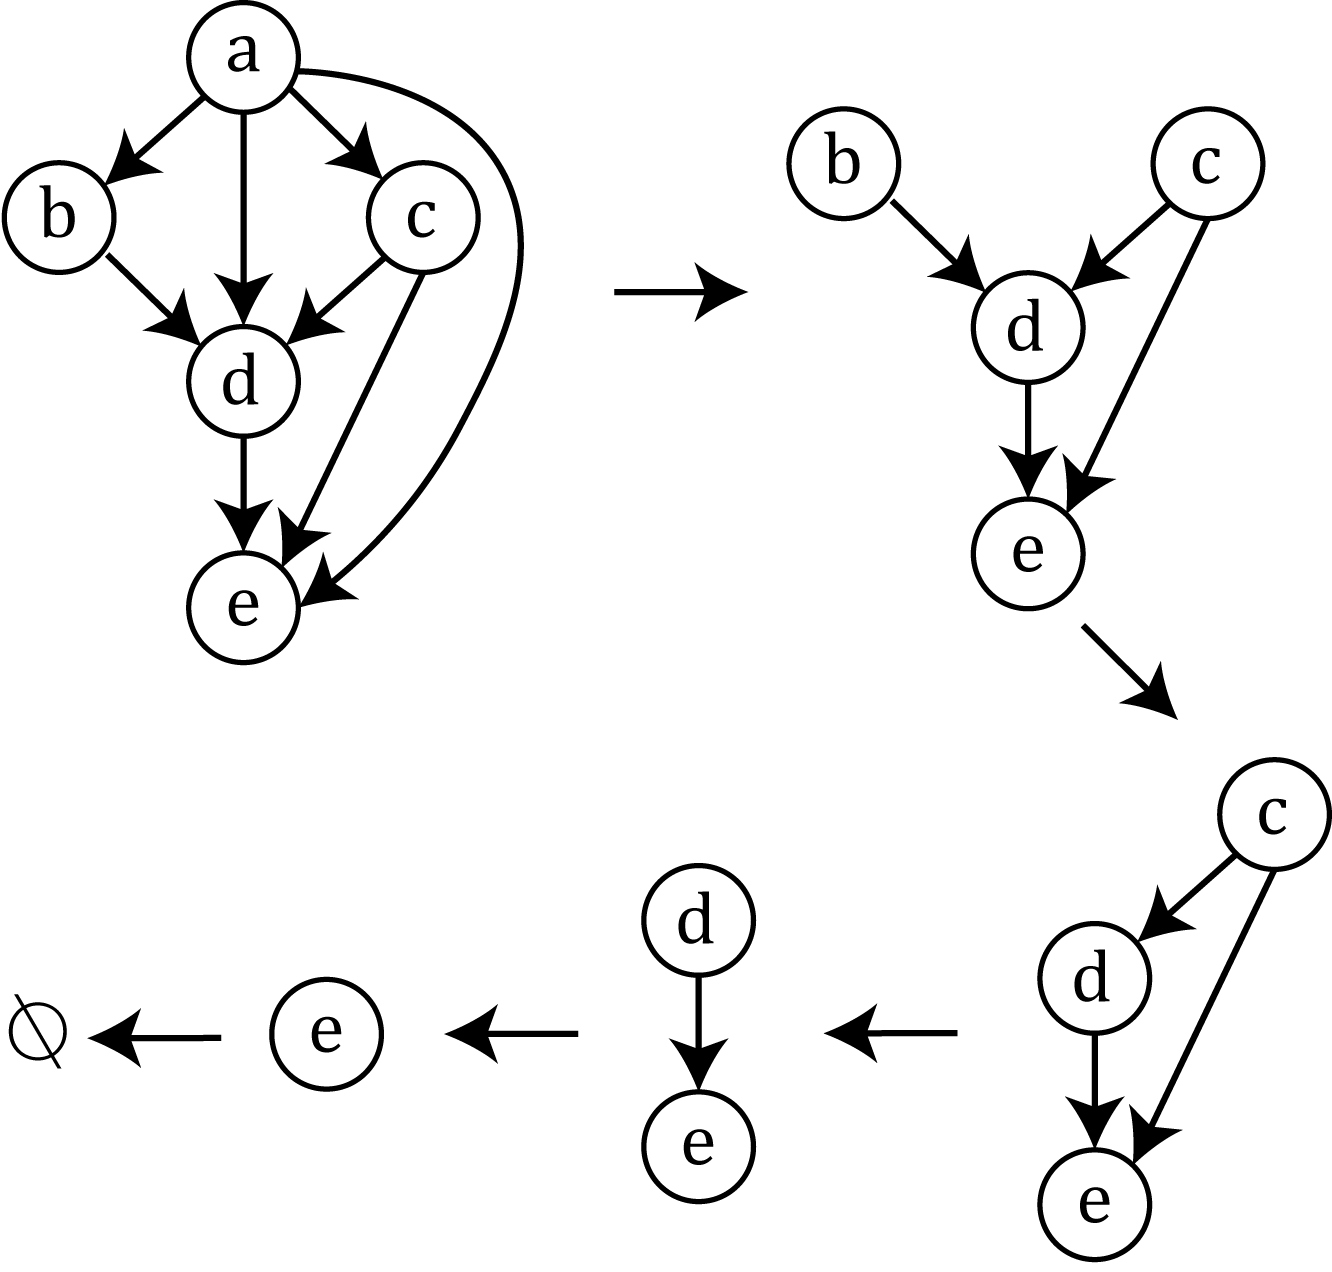
\includegraphics[width=5cm]{pics/38_3}
            \centering
    \end{figure}
    \[M_0 = \varnothing,\qq M_2 = \{a,b,c,d,e\}\]
    \begin{enumerate}
      \item $N_a^+ = \varnothing \Ra a \ra M_0$
      \item $N_b^+ = \varnothing \Ra b \ra M_0$
      \item $N_c^+ = \varnothing \Ra c \ra M_0$
      \item $N_d^+ = \varnothing \Ra d \ra M_0$
      \item $N_e^+ = \varnothing \Ra e \ra M_0$
    \end{enumerate}
  \end{example}
\end{document}
